\subsection{Exercise 1}
\begin{figure}[H]
    \centering
    \begin{subfigure}[t]{0.5\textwidth}
        \centering
        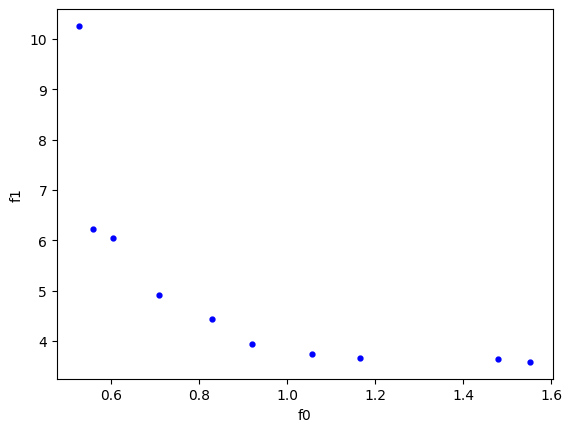
\includegraphics[width=\linewidth]{images/lab5/pfront_unconstrained_base.png}
        \caption{unconstrained (population of 10 for \\10 generations)}
    \end{subfigure}%
    \begin{subfigure}[t]{0.5\textwidth}
        \centering
        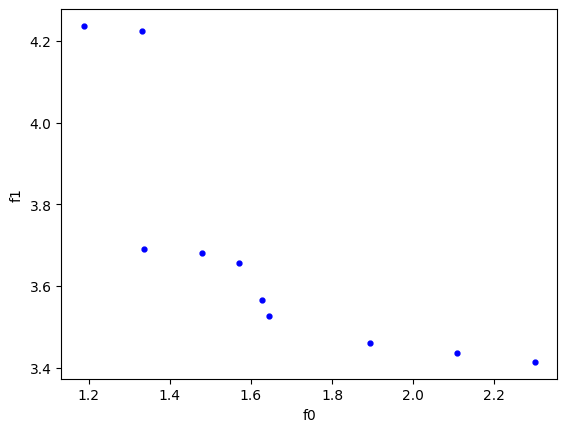
\includegraphics[width=\linewidth]{images/lab5/pfront_constrained_base.png}
        \caption{constrained (population of 10 for 10 generations)}
    \end{subfigure}
\end{figure}


\begin{figure}[H]
    \centering
    \begin{subfigure}[t]{0.5\textwidth}
        \centering
        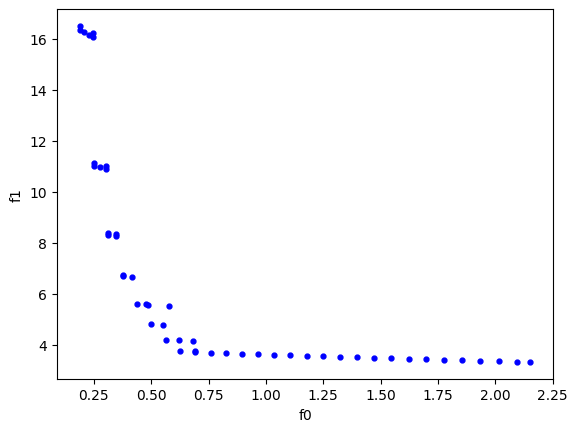
\includegraphics[width=\linewidth]{images/lab5/pfront_unconstrained_high.png}
        \caption{unconstrained (population of 50 \\ for 250 generations)}
    \end{subfigure}%
    \begin{subfigure}[t]{0.5\textwidth}
        \centering
        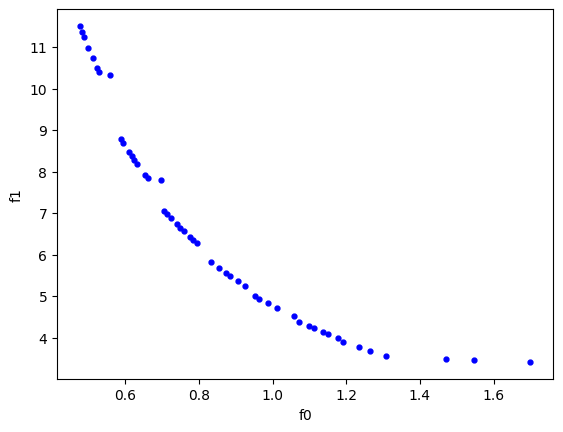
\includegraphics[width=\linewidth]{images/lab5/pfront_constrained_high.png}
        \caption{constrained (population of 50 for 250 generations)}
    \end{subfigure}
\end{figure}
In the unconstrained scenario we can see that we can achieve better values for both function while in the constrained scenario we can't reach them even with a larger population and number of generations, probably due to these values being in an unfeasible area for the constrained scenario 

It's interesting to notice that in the constrained scenario we have can see we have better crowding than the unconstrained (maybe due to how some constraints shape the feasible space 

\subsection{Exercise 2}
\subsubsection{Rosenbrock}
Compare with sol in lab2
\subsubsection{Townsend}
\begin{figure}[H]
    \centering
    \begin{subfigure}[t]{0.5\textwidth}
        \centering
        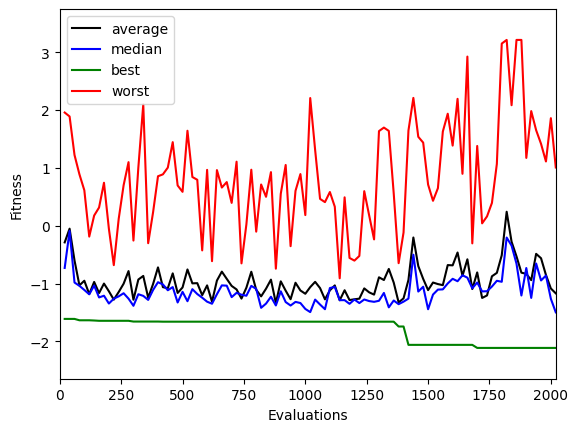
\includegraphics[width=\linewidth]{images/lab5/townsend_fitness.png}
    \end{subfigure}%
    \begin{subfigure}[t]{0.5\textwidth}
        \centering
        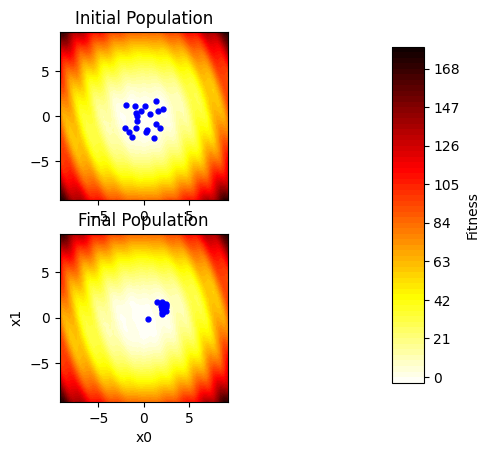
\includegraphics[width=\linewidth]{images/lab5/townsend_population.png}
    \end{subfigure}
\end{figure}
Best Individual: [2.03889998 1.31315151] \\
Best Fitness: -2.111579385394471 \\
f  = -2.5435914877447443 \\
g1 = 0.43201210235027343 \\
(unfeasible)\\
Solution really close to the global minimum but unfeasible


\subsection{General questions}
What do you think is the most efficient way to handle constraints in EAs?


Do you think that the presence of constraints makes the search *always* more difficult? Can you think of cases in which the constraints could actually make the search easier?